\problemname{Göngutúr}


Inga litla er svakalega dugleg, en hún fer út að ganga á hverjum einasta
morgni. Síminn hennar, sem hún hefur alltaf meðferðis, skráir niður leiðina sem
hún gengur. Núna er Inga komin heim og hana langar að vita hversu langt hún
gekk. Hjálpið Ingu með því að skrifa forrit sem reiknar hversu langt hún gekk.

Síminn skráir niður hnit Ingu á nokkurra sekúndna millibili. Hnitin eru gefin
upp í tvívíðu kartesku hnitakerfi, og má því ímynda sér að Inga gangi um
á flötu plani. Öll hnit eru gefin upp í metrum.

Eitt dæmi um göngutúr er sýndur á eftirfarandi mynd. Þar labbaði Inga $3$
metra.

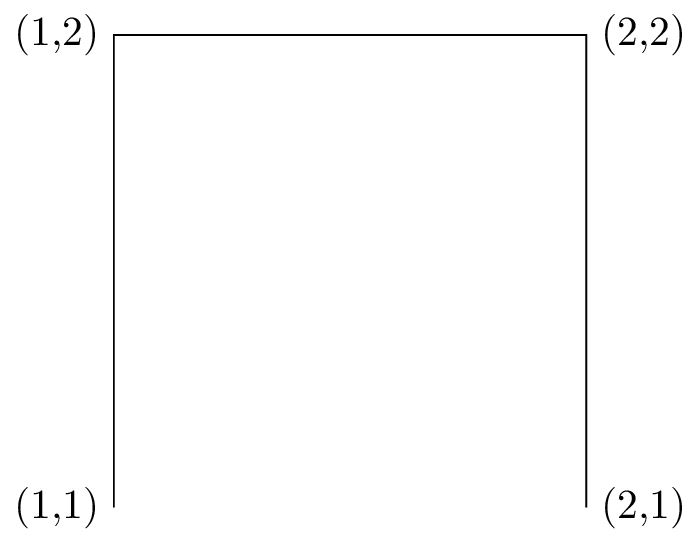
\includegraphics[scale=0.4]{path.png}

Fyrsta lína inntaks inniheldur heiltöluna $n$. Þar eftir fylgja $n$ línur, sem
hver inniheldur tvær kommutölur aðskildar með bili. Þessi $n$ pör af tölum
tákna hnitin sem síminn hennar gaf upp, í sömu röð. Úttak á að innihalda eina
kommutölu sem táknar hversu langt Inga litla gekk. Skekkja í svari má ekki vera
stærri en $10^{-3}$.

